\newpage
\subsection{UC4 - Modifica Grafico}
\label{sub:uc2}

%TODO: Add correct image
\begin{figure}[h]
    \centering
    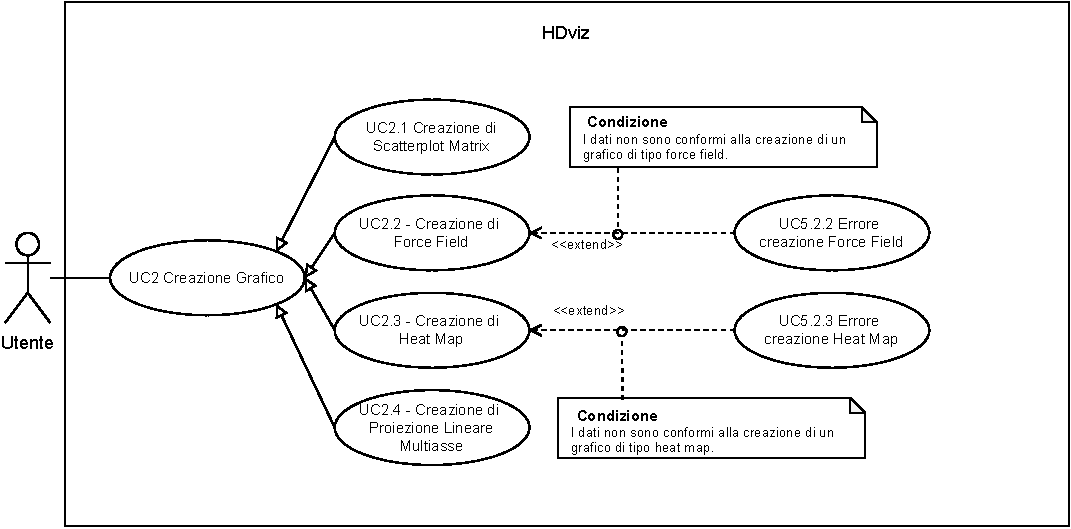
\includegraphics[width=0.8\textwidth]{componenti/casi-duso/diagrammi/UC2.pdf}
    \caption{Diagramma rappresentante UC2}
    \label{fig:UC2}
\end{figure}


\begin{itemize}
    \item \textbf{Descrizione}: L’utente modifica la visualizzazione del grafico precedentemente costruito
                                e ne vede le modifiche.
	
    \item \textbf{Attore primario}: Utente.
    
    \item \textbf{Precondizione}:   Nel programma è stato importato un dataset dotato di metatag per ogni
                                    colonna dei dati ed è stato costruito un grafico di una tipologia scelta dall'utente.

    \item \textbf{Postcondizione}:  Viene aggiornato il grafico costruito e visualizzato con i nuovi parametri.

	\item \textbf{Scenario principale}:
		\begin{enumerate}
			\item L'utente decide di modificare il grafico corrente.
			\item All'utente vengono fornite le opzioni del tipo di grafico che è stato costruito precedentemente.
        \end{enumerate}

    \item \textbf{Generalizzazioni}:
        \begin{itemize}
            \item Modifica del grafico Scatterplot Matrix (UC4.1)
            \item Modifica del grafico Force Field (UC4.2)
            \item Modifica del grafico Heat Map (UC4.3)
            \item Modifica del grafico Proiezione Lineare Multiasse (UC4.4)
        \end{itemize}
\end{itemize}


\subsection{UC4.1 Modifica Scatterplot Matrix}

\subsection{UC4.2 Modifica Force Field}